\section{Results}
\label{sec:results}

\subsection{The decoders use the neural signal}
\label{sec:res-decoders}
On Brain-to-Text '25, our phoneme-to-word decoder reached WER 0.149 with the right sentence first for 39\% of test trials, and the published decoder WER 0.043 with 81\%. On sEMG, balanced key accuracies (0.367, 0.240, 0.226) were well above chance (0.037), and after the LM the right sentence was first for 46\%, 12\% and 4\% of composed sentences. Our asynchronous MEG decoder reached a test CER of 0.475 (shuffled MEG 0.760, zero input 0.925; three seeds and controls: \cref{tab:decoders,tab:seeds}), but its top-1 sentence was right for only 2 of 637 instances.

\subsection{Time-ordered deployment: the guaranteed rule held across days}
\label{sec:res-forward}
\Cref{tab:forward} and \cref{fig:deploy}a give the time-ordered tests on Brain-to-Text '25, where calibration always came before the test data. Under the LTT max rule, the pooled wrong-commit rate was 0.010--0.027 in every design, on both decoders. It was above $\alpha$ on 0--2 of 10--13 test days, and no day had a CP lower bound above $\alpha$; the highest single day was 0.060. With one previous day as calibration (V1), it committed 11\% (ours) and 32\% (published) of trials, and 20\% and 5\% of these commits were wrong. The plug-in rule was above $\alpha$ on up to 6 of 10 days, and in three of the four designs one day had a CP lower bound above $\alpha$ (ours). CRC with the max rule lay between the two. With the guard off (plain threshold), LTT max was above $\alpha$ on 0 of 12 days in V1 (pooled 0.018 ours, 0.010 published) (\cref{tab:forward-full}). Twelve test days can neither confirm nor exclude control at level $\delta$ per day: 2 of 12 days has a CP interval of 0.02--0.48.

\begin{table}[t]
  \centering
  \caption{\textbf{Time-ordered (forward-chaining) deployment on Brain-to-Text '25} (guard on). Calibration data always come before the test data. Days $>\alpha$: test days with a wrong-commit rate above $\alpha = 0.05$ (none had a CP lower bound above $\alpha$ under LTT max). Pooled: wrong-commit rate over all test trials of the design, with exact CP 95\% CI. Commit, EAC: pooled. Joint LTT: commit rate with $\beta = 0.10$. Guard off and all rules: \cref{tab:forward-full}.}
  \label{tab:forward}
  \small
  \begin{adjustbox}{max width=\linewidth}\begin{tabular}{@{}lllllllll@{}}
    \toprule
    & & \textbf{Plug-in} & \textbf{CRC max} & \multicolumn{4}{c}{\textbf{LTT max (primary)}} & \textbf{Joint LTT} \\
    \cmidrule(lr){5-8}
    \textbf{Decoder} & \textbf{Design (test days)} & \textbf{Days $>\alpha$} & \textbf{Days $>\alpha$} & \textbf{Days $>\alpha$} & \textbf{Pooled [CP95]} & \textbf{Commit} & \textbf{EAC} & \textbf{Commit} \\
    \midrule
    Ours & V1: previous day (12) & 5 & 4 & \textbf{2} & 0.022 \ci{0.015}{0.031} & 0.11 & 0.20 & 0 \\
     & V4: two previous days (11) & 5 & 4 & \textbf{0} & 0.027 \ci{0.019}{0.037} & 0.14 & 0.20 & 0 \\
     & V2: all earlier days (10) & 6 & 4 & \textbf{1} & 0.027 \ci{0.019}{0.038} & 0.15 & 0.18 & 0 \\
     & V3: session start (13) & 5 & 3 & \textbf{2} & 0.015 \ci{0.008}{0.026} & 0.09 & 0.17 & 0 \\
    Published gate & V1: previous day (12) & 1 & 1 & \textbf{0} & 0.016 \ci{0.010}{0.024} & 0.32 & 0.05 & 0 \\
     & V4: two previous days (11) & 0 & 0 & \textbf{0} & 0.020 \ci{0.013}{0.029} & 0.35 & 0.06 & 0.04 \\
     & V2: all earlier days (10) & 0 & 0 & \textbf{0} & 0.023 \ci{0.016}{0.033} & 0.29 & 0.08 & 0.06 \\
     & V3: session start (13) & 1 & 1 & \textbf{1} & 0.010 \ci{0.004}{0.020} & 0.19 & 0.05 & 0 \\
    \bottomrule
  \end{tabular}\end{adjustbox}
\end{table}

\begin{figure}[t]
  \centering
  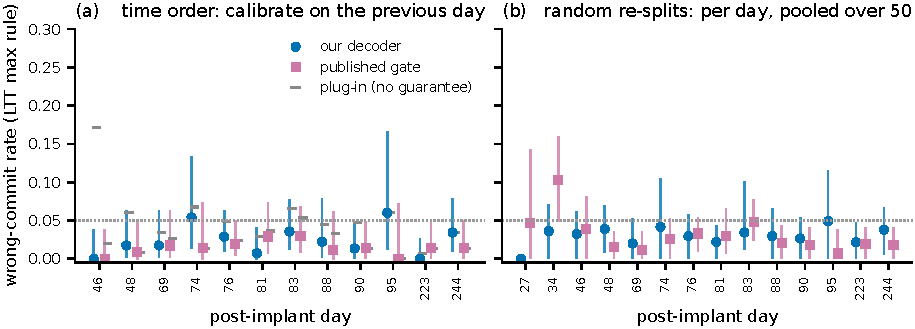
\includegraphics[width=\linewidth]{fig_deploy.pdf}
  \caption{\textbf{The guaranteed rule across days} (Brain-to-Text '25, guard on, LTT max rule; dotted line: $\alpha = 0.05$). (a)~Time order (V1: fit on days $1..k{-}2$, calibrate on day $k{-}1$, test on day $k$): wrong-commit rate per test day with exact CP 95\% CIs; small grey markers: plug-in rule. (b)~Random re-splits: wrong-commit rate per day pooled over 50 re-splits; bars: 5th--95th percentile over re-splits. The bound covers the mix of days; on the published gate, day 34 ran at about $2\alpha$.}
  \label{fig:deploy}
\end{figure}

\subsection{Random re-splits and the scope of the guarantee}
\label{sec:res-resplits}
\label{sec:res-perday}
Over 50 random re-splits (\cref{tab:repeat}), the LTT max rule gave mean wrong-commit rates of 0.030 (our decoder) and 0.031 (published gate). It exceeded $\alpha$ on the test set in 4/50 = 0.08 \ci{0.02}{0.19} and 1/50 = 0.02 \ci{0.001}{0.11} of re-splits. Fifty re-splits cannot show that this share is at most $\delta = 0.1$, and the test-set share includes test-sampling noise. The exact population exceedance, which LTT bounds, was 0.026 and 0.014. CRC met its own target, the mean (0.046 and 0.049), and, as designed, many single re-splits were above $\alpha$ (34\% and 42\%). LTT max was never above $\alpha$ in a re-split where CRC max was not; with 50 re-splits this difference was significant only on the published gate (exact McNemar $p = 0.25$ and $0.031$; with 200 re-splits $p < 10^{-6}$ on both, \cref{app:population}). With the guard off, LTT max exceeded $\alpha$ in 0 of 50 re-splits on both decoders. On sEMG, LTT max committed 9\% and 2\% of sentences (session-calibrated, cross-session; mean wrong-commit 0.011 and 0.006) and never exceeded $\alpha$; on cross-session, 34\% of re-splits never committed, and the cross-subject decoder never committed.

Per day, the risk was not controlled (\cref{fig:deploy}b, \cref{tab:perday}). On the published gate, day 34 (about 50 test trials per re-split) had a pooled wrong-commit rate of 0.102 under LTT max, and it was above $\alpha$ in 94\% of re-splits; in fixed splits A and B it had 8 wrong commits in 50 trials (0.16, CP95 \ci{0.07}{0.29}). The other days had 0.007--0.048, and our decoder 0.000--0.049 on every day. LTT bounds the risk over the mix of days that the calibration set comes from, not each day. Per-day (Mondrian) LTT with a quarter of each day as calibration was feasible only on the one day with at least 45 calibration items, and committed nothing on the other 13 days.

The guaranteed rule was faster than the same fitted policy without commits in every re-split: by $+0.114$ \ewpm{} (Monte-Carlo SE 0.005) on our decoder and $+0.510$ (SE 0.007) on the published gate, about 1\% and 3\%. On the fixed test set, the paired gains were $+0.058$ \ci{0.034}{0.090} and $+0.125$ \ci{0.077}{0.188} (ours, splits A and B) and $+0.537$ \ci{0.439}{0.636} and $+0.567$ \ci{0.456}{0.694} (published).

\begin{table}[t]
  \centering
  \caption{\textbf{Random re-splits} (50; exchangeable by construction, so a check of the theorems on one data pool, not a deployment test). Wrong-commit: mean test rate (5th--95th percentile over re-splits); $>\alpha$: share of re-splits with a test rate above $\alpha$, with exact CP 95\% CI; Pop.: share of with-replacement calibration draws whose exact population risk exceeds $\alpha$ (\cref{app:population}); Commit: mean; EAC: pooled; Gain: mean paired \ewpm{} gain over the same fitted policy without commits. The spread is split-to-split variation in one data set, not a CI for new data. sEMG rows: \cref{tab:repeat-full}.}
  \label{tab:repeat}
  \small
  \begin{adjustbox}{max width=\linewidth}\begin{tabular}{@{}lllllll@{}}
    \toprule
    \textbf{Rule} & \textbf{Wrong-commit} & $\boldsymbol{>\alpha}$ \textbf{[CP95]} & \textbf{Pop.} & \textbf{Commit} & \textbf{EAC} & \textbf{Gain} \\
    \midrule
    \multicolumn{7}{@{}l}{\textit{Brain-to-Text '25, our decoder}} \\
    plug-in (fit-A) & 0.044 (0.021--0.072) & 0.34 \ci{0.21}{0.49} & --- & 0.19 & 0.24 & $+0.132$ \\
    CRC, pure & 0.046 (0.026--0.068) & 0.34 \ci{0.21}{0.49} & 0.39 & 0.19 & 0.24 & --- \\
    CRC, max rule & 0.037 (0.021--0.059) & 0.14 \ci{0.06}{0.27} & 0.17 & 0.17 & 0.22 & $+0.125$ \\
    \textbf{LTT, max rule} & \textbf{0.030} (0.016--0.052) & \textbf{0.08} \ci{0.02}{0.19} & 0.026 & 0.15 & 0.21 & $+0.114$ \\
    LTT, max rule, guard off & 0.031 (0.013--0.043) & 0.00 \ci{0}{0.07} & --- & 0.14 & 0.21 & $+0.106$ \\
    \midrule
    \multicolumn{7}{@{}l}{\textit{Brain-to-Text '25, published gate}} \\
    plug-in (fit-A) & 0.039 (0.021--0.060) & 0.22 \ci{0.12}{0.36} & --- & 0.43 & 0.09 & $+0.564$ \\
    CRC, pure & 0.049 (0.029--0.075) & 0.42 \ci{0.28}{0.57} & 0.40 & 0.48 & 0.10 & --- \\
    CRC, max rule & 0.036 (0.021--0.055) & 0.14 \ci{0.06}{0.27} & 0.074 & 0.42 & 0.09 & $+0.546$ \\
    \textbf{LTT, max rule} & \textbf{0.031} (0.020--0.047) & \textbf{0.02} \ci{0.001}{0.11} & 0.014 & 0.39 & 0.08 & $+0.510$ \\
    LTT, max rule, guard off & 0.024 (0.018--0.031) & 0.00 \ci{0}{0.07} & --- & 0.36 & 0.07 & $+0.471$ \\
    \bottomrule
  \end{tabular}\end{adjustbox}
\end{table}

\subsection{Fixed test sets; sEMG and MEG as format and safety checks}
\label{sec:res-main}
On the fixed test set (\cref{tab:main}), always committing sent wrong text for 0.610 of trials on our decoder and 0.194 on the published sentence, because one wrong word makes a sentence wrong. The guaranteed rule gave 0.025 and 0.052 (splits A and B) on our decoder and 0.029 and 0.031 on the published gate. The plug-in layer fitted on all fit trials gave 0.059 \ci{0.045}{0.070} on our decoder, above $\alpha$. The difference to the fit-A rows comes from the policy grid fitted on fit-A, not from the risk control: in split A, CRC and LTT were not binding (\cref{app:full}). On sEMG, the layer cut the wrong-commit rate from 0.541, 0.882 and 0.962 to 0.004, 0.004 and 0, committing 21, 10 and 0 of 551 sentences; the guaranteed rule gave the same rows. On MEG the layer committed nothing (0 of 637, one-sided 95\% upper bound 0.0047) and equals always offering; no guarantee for new sentences is possible on these data, because a sentence-level LTT needs at least 45 calibration sentences and the data set has 17 test sentences (\cref{app:meg}). Only the session-calibrated sEMG decoder clearly beat gaze typing \ci{+2.71}{+4.91}; on the 256 sEMG test sentences without a near variant in the LM text, speeds were lower and gaze typing beat the cross-subject decoder (\cref{app:leakage}).

\begin{table}[t]
  \centering
  \caption{\textbf{Safety and speed on the fixed test sets.} Plug-in: full fit, no guarantee. Guaranteed rule (the frozen configuration of \cref{sec:discussion}): fit-A pipeline, guard, clean calibration, LTT max rule (B2T '25: splits A and B, $n_{\mathrm{cal}} = 401$; sEMG: 143). Guard off: the same with the plain threshold. EAC: error among commits (wrong/commits in brackets; count only if fewer than 30 commits). Silent: uncorrected wrong final texts per item. 95\% cluster-bootstrap CIs over days (B2T '25), participants (sEMG) or sentences $\times$ participants (MEG), conditional on the fitted pipeline and threshold. Zero rates: one-sided 95\% upper bounds 0.0037 (816 items), 0.0054 (551) and 0.0047 (637). All policies: \cref{tab:full}.}
  \label{tab:main}
  \small
  \begin{adjustbox}{max width=\linewidth}\begin{tabular}{@{}lllllll@{}}
    \toprule
    \textbf{Device} & \textbf{Policy} & \textbf{\ewpm{} [CI]} & \textbf{Wrong-commit [CI]} & \textbf{Commit} & \textbf{EAC} & \textbf{Silent} \\
    \midrule
    B2T '25, our decoder & always commit & 11.45 \ci{10.70}{12.31} & 0.610 \ci{0.568}{0.647} & 1.00 & 0.61 & 0.044 \\
     & always offer & 11.37 \ci{10.67}{12.17} & 0 & 0 & --- & 0 \\
     & plug-in & 11.55 \ci{10.83}{12.34} & 0.059 \ci{0.045}{0.070} & 0.23 & 0.25 (48/189) & 0.003 \\
     & \textbf{guaranteed rule, A} & 11.48 \ci{10.79}{12.29} & \textbf{0.025} \ci{0.015}{0.035} & 0.10 & 0.24 (20/82) & 0.001 \\
     & \textbf{guaranteed rule, B} & 11.54 \ci{10.83}{12.34} & \textbf{0.052} \ci{0.043}{0.059} & 0.19 & 0.27 (42/157) & 0.003 \\
     & guard off, A & 11.55 \ci{10.83}{12.39} & 0.040 \ci{0.030}{0.051} & 0.18 & 0.22 (33/149) & 0 \\
     & guard off, B & 11.53 \ci{10.82}{12.37} & 0.029 \ci{0.021}{0.038} & 0.15 & 0.20 (24/120) & 0 \\
    B2T '25, published & always commit & 19.61 \ci{17.81}{21.32} & 0.194 \ci{0.146}{0.253} & 1.00 & 0.19 & 0.025 \\
     & always offer & 18.11 \ci{16.59}{19.57} & 0 & 0 & --- & 0 \\
     & plug-in & 18.77 \ci{17.13}{20.35} & 0.044 \ci{0.027}{0.068} & 0.47 & 0.09 (36/386) & 0.004 \\
     & \textbf{guaranteed rule, A} & 18.65 \ci{17.04}{20.20} & \textbf{0.029} \ci{0.013}{0.050} & 0.40 & 0.07 (24/329) & 0.001 \\
     & \textbf{guaranteed rule, B} & 18.68 \ci{17.06}{20.23} & \textbf{0.031} \ci{0.014}{0.052} & 0.42 & 0.07 (25/339) & 0.003 \\
     & guard off, A & 18.63 \ci{17.03}{20.18} & 0.027 \ci{0.016}{0.040} & 0.39 & 0.07 (22/319) & 0.001 \\
     & guard off, B & 18.63 \ci{17.02}{20.18} & 0.025 \ci{0.014}{0.038} & 0.39 & 0.06 (20/316) & 0.001 \\
    B2T '25 & gaze typing & 4.08 \ci{4.05}{4.12} & 0 & --- & --- & 0 \\
    \midrule
    sEMG session-cal. & always commit & 7.81 \ci{6.66}{9.04} & 0.541 \ci{0.463}{0.621} & 1.00 & 0.54 & 0.060 \\
     & \textbf{guaranteed rule} & 7.98 \ci{6.95}{9.11} & \textbf{0.004} \ci{0}{0.009} & 0.04 & 2/21 & 0 \\
    sEMG cross-session & always commit & 4.10 \ci{3.56}{4.73} & 0.882 \ci{0.831}{0.928} & 1.00 & 0.88 & 0.149 \\
     & \textbf{guaranteed rule} & 4.68 \ci{4.19}{5.25} & \textbf{0.004} \ci{0}{0.009} & 0.02 & 2/10 & 0 \\
    sEMG cross-subject & always commit & 3.53 \ci{3.19}{3.90} & 0.962 \ci{0.942}{0.981} & 1.00 & 0.96 & 0.167 \\
     & \textbf{guaranteed rule} & 4.08 \ci{3.82}{4.37} & \textbf{0} & 0 & --- & 0 \\
    sEMG & gaze typing & 4.27 \ci{4.22}{4.32} & 0 & --- & --- & 0 \\
    \midrule
    MEG (asynchronous) & always commit & 2.58 \ci{2.31}{2.88} & 0.997 \ci{0.987}{1.000} & 1.00 & 1.00 & 0.235 \\
     & trust (= always offer) & 3.20 \ci{3.01}{3.44} & 0 & 0 & --- & 0 \\
    MEG & gaze typing & 3.15 \ci{3.02}{3.31} & 0 & --- & --- & 0 \\
    \bottomrule
  \end{tabular}\end{adjustbox}
\end{table}

\subsection{A guaranteed error among commits of 10\% almost never commits}
\label{sec:res-selective}
The marginal rules let a weak decoder commit text that is often wrong: 21\% of the guaranteed rule's commits on our decoder (\cref{tab:repeat}). Joint LTT bounds both risks (\cref{tab:selective}). With $\beta = 0.10$ it committed nothing on our decoder, sEMG and MEG, nothing in either fixed split, and nothing in any time-ordered design with one day of calibration. Over random re-splits of the published gate, it committed 7.2\% of sentences on average (none in 76\% of re-splits), with an error among commits of 0.059. With $\beta = 0.20$, it committed 32\% of published sentences with an error among commits of 0.062, and 0.32 in fixed split A (error among commits 0.057 \ci{0.032}{0.093}); our decoder still committed 0.1\%. LTT-sel, which bounds only the selective risk, committed 56\% of published sentences at $\beta = 0.20$, but its marginal rate (0.074) exceeded $\alpha$ in 76\% of re-splits. The limit is the calibration size: an exact bound on the error among commits needs many calibration commits.

\begin{table}[t]
  \centering
  \caption{\textbf{Controlling the error among commits} (B2T '25 published gate, 50 random re-splits, guard on, $\delta = 0.1$; test set). Commit: mean (share of re-splits with no commit); EAC: pooled error among commits; $>\beta$: committing re-splits with EAC above $\beta$; Marginal: mean wrong-commit rate ($>\alpha$: share of re-splits above $\alpha$). Joint LTT: both targets, fixed grid, Bonferroni (valid for both). LTT-sel: selective target only. SGR: bisection \citep{geifman2017selective}. Our decoder: joint LTT commits nothing at $\beta = 0.10$ and 0.1\% at $\beta = 0.20$; sEMG and MEG: no commits at any $\beta$.}
  \label{tab:selective}
  \small
  \begin{adjustbox}{max width=\linewidth}\begin{tabular}{@{}llllllll@{}}
    \toprule
    $\boldsymbol\beta$ & \textbf{Rule} & \textbf{Commit (none)} & \textbf{EAC} & $\boldsymbol{>\beta}$ & \textbf{Marginal} & $\boldsymbol{>\alpha}$ & \textbf{\ewpm{}} \\
    \midrule
    0.10 & \textbf{joint LTT} & 0.072 (0.76) & 0.059 & 0 of 12 & 0.004 & 0 & 18.07 \\
         & LTT-sel & 0.072 (0.76) & 0.059 & 0 of 12 & 0.004 & 0 & 18.07 \\
         & SGR & 0.112 (0.64) & 0.069 & 0 of 18 & 0.008 & 0 & 18.12 \\
    0.20 & \textbf{joint LTT} & 0.318 (0.02) & 0.062 & 0 of 49 & 0.020 & 0 & 18.39 \\
         & LTT-sel & 0.564 (0) & 0.131 & 0 of 50 & 0.074 & 0.76 & 18.72 \\
         & SGR & 0.617 (0) & 0.142 & 0 of 50 & 0.088 & 0.92 & 18.79 \\
    --- & LTT max rule (marginal only) & 0.392 (0) & 0.078 & --- & 0.031 & 0.02 & 18.49 \\
    --- & no commits & 0 (1) & --- & --- & 0 & 0 & 17.98 \\
    \bottomrule
  \end{tabular}\end{adjustbox}
\end{table}

\subsection{Controls: without the guard, the layer commits no-information streams}
\label{sec:res-null}
Always committing wrote a sentence for every control stream. With the guard, the guaranteed rule (split A) committed none of the 300 frame-shuffled and none of the 300 uniform streams on either Brain-to-Text '25 decoder (one-sided 95\% upper bound 0.0099), while it committed 29 (ours) and 115 (published) of the 300 matched real trials; the full-fit layer also committed none, and so did sEMG (0 of 200 sentences per control; bound 0.015) (\cref{fig:null}). Without the guard, our decoder committed 198 of 300 uniform streams under the plain threshold with the LTT max rule (all 198 commits wrong) and 3 of 300 frame-shuffled streams. A uniform stream gives flat phoneme posteriors; the word decoder then returns a fluent LM sentence with a high calibrated $\hat p_{\mathrm{top1}}$, and the calibration data, which contain only real streams, cannot detect this. The published gate, sEMG and MEG committed no control stream with or without the guard. On real data, in contrast, the guard did not lower wrong commits. Without it, the full-fit wrong-commit rate on our decoder fell from 0.059 to 0.036 (paired \ci{-0.035}{-0.011}; sign test over days $p = 0.021$). In the re-splits, the time-ordered tests and the fixed splits, the rates without the guard were lower on the published gate in 6 of 7 comparisons and mixed on our decoder (lower in 2, similar in 2, higher in 3; fixed split A: 0.040 against 0.025) (\cref{tab:repeat,tab:main,tab:forward-full}). A commit rule therefore needs an input-validity check that real calibration data do not test; in these fits our guard was one such check, but not in every fit: the grid value $r_{\max} = 1.0$ switches its limit off (\cref{app:guardlimit}). A better check is open. Given the real stream of another sentence (intent mismatch), the layer committed at the matched rate on our decoder: nothing in the stream reveals the intent. The published gate committed none of these 300 streams (\cref{tab:controls}).

\subsection{Speed depends on the user model; wrong-commit rates do not}
\label{sec:res-user}
\Cref{fig:usermodel} refits every policy (plug-in layer) under eight user-model variants. The layer was at least as fast as always offering in every variant and condition. Always committing was faster than the layer on the published gate in all 9 variants (by 0.46--1.47 \ewpm{}, every CI below 0) and on our decoder in 5 of 9 (CI below 0 in 1, above 0 in 3). Gaze typing with word completion had a higher point value than the layer in every variant on MEG and on the two weaker sEMG decoders. The wrong-commit rate of the refitted layer was at most 0.059 in all 54 condition--variant pairs.

\begin{figure}[t]
  \centering
  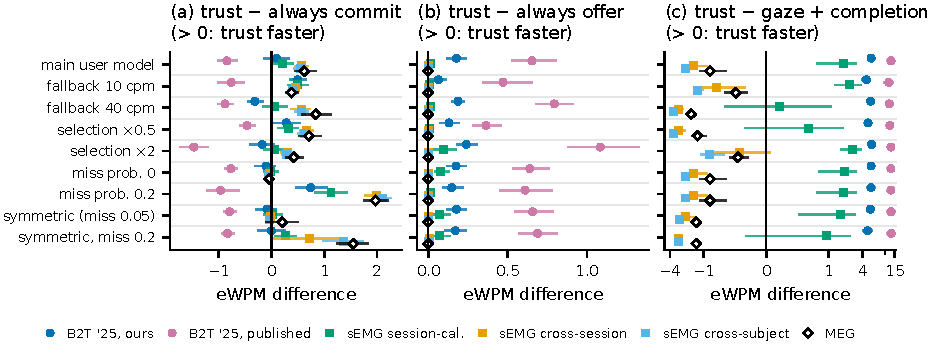
\includegraphics[width=\linewidth]{fig_user_model.pdf}
  \caption{\textbf{User-model sensitivity} (plug-in layer, full fit; not the guaranteed rule). Paired \ewpm{} difference between the trust layer and (a)~always committing, (b)~always offering and (c)~gaze typing with word completion (symmetric-log axis), all policies refitted under each variant (rows); values above 0 mean that the layer is faster. 95\% cluster-bootstrap CIs at the primary unit.}
  \label{fig:usermodel}
\end{figure}

\subsection{Calibration and the other components}
\label{sec:res-ablation}
Sentence ECE fell from 0.448 \ci{0.419}{0.475} to 0.067 \ci{0.065}{0.104} on our intracortical decoder and from 0.102 \ci{0.058}{0.161} to 0.058 \ci{0.044}{0.090} on the published gate (percentile CIs; binned ECE is biased upwards, so an interval can lie beside its point value). The calibrated $\hat p_{\mathrm{top1}}$ predicted a wrong top sentence with AUROC 0.797 \ci{0.773}{0.819} (ours), 0.710 \ci{0.678}{0.744} (published) and 0.828, 0.755 and 0.674 on sEMG (\cref{app:ece}); the MEG AUROC is not informative (2 right sentences). The frame temperature raised the ECE of per-frame phoneme peaks (0.090 to 0.130) although it minimises their cross-entropy; we did not resolve why, but the two criteria differ (cross-entropy at aligned peaks with blank targets for inserted peaks, ECE of the arg-max confidence). Without the sentence temperature, wrong commits rose on 4 of 6 conditions (\cref{tab:ablation}). Calibrating pure CRC on data that had also fitted the pipeline raised the test rate on our decoder by $+0.009$ (day-jackknife 95\% CI \ci{+0.005}{+0.013}; Holm-adjusted $p = 0.004$ over 12 comparisons), conditional on this data pool; no other condition showed an effect after Holm, and with 200 re-splits the effect was $+0.003$ (\cref{tab:reuse}). As the threshold varies, the published decoder can commit about half of its sentences at the 0.05 marginal level and our decoder about a fifth (\cref{fig:calib}).
